\section{Test Results}

In order to test the performance of time and frequency transfer, the 
test setup depicted in \figurename~\ref{fig:testSetup} was assembled.
The system consists of 4 switches connected with 5km bare fiber rolls in 
a daisy chain (15~km total). Varying operating conditions were simulated
by heating the fiber with a hot air gun. 


\begin{figure}[!t]
\centering
%\includegraphics[width=2.0in]{fig/measSystem.ps}
\includegraphics[width=1.6in]{measurements/measSystem.pdf}
\caption{Test setup.}
\label{fig:testSetup}
\end{figure}

%\subsection{Syntonization}

The frequency transfer performance was evaluated using an Agilent E5052B signal source analyzer. 
A cesium clock served as a source of 10~MHz reference frequency for the master.
The Power Spectral Density (PSD) of the phase noise of the master and each slave 
REF clocks was determined. The integrated jitter from 10Hz to 40~MHz measured on each 
slave is presented in Table~\ref{tab:freqTransfer}. The jitter on a single link is below 2~ps. 
%the accumulation effect of cascaded switches can be observed.

The accuracy \modified{and precision} of synchronization %was 
were characterized by measuring the skew between 
the master and each slave clock signal over a period of 1 hour with a LeCroy oscilloscope
(Table~\ref{tab:freqTransfer}). A histogram of master-slave offsets constructed from the obtained
samples is depicted in \figurename~\ref{fig:offset}. The single link skew is
well below 1~ns. In this particular case, the skews of the first and second link cancel,
therefore the skew between the master and the last slave is below 200~ps. However, if the
cancellation did not take place, the accumulated skew would be still below 0.5~ns. The varying
conditions introduce only a transient increase of the skew's standard deviation (sdev) of 
$\sim$~5~ps. This is a consequence of the purposely %very 
low exchange-rate of PTP messages (1~s), compared
to the fast heating provided by the hot air gun.
\begin{figure}[!t]
\centering
%\includegraphics[width=2.3in]{fig/cascadedMeas.eps}
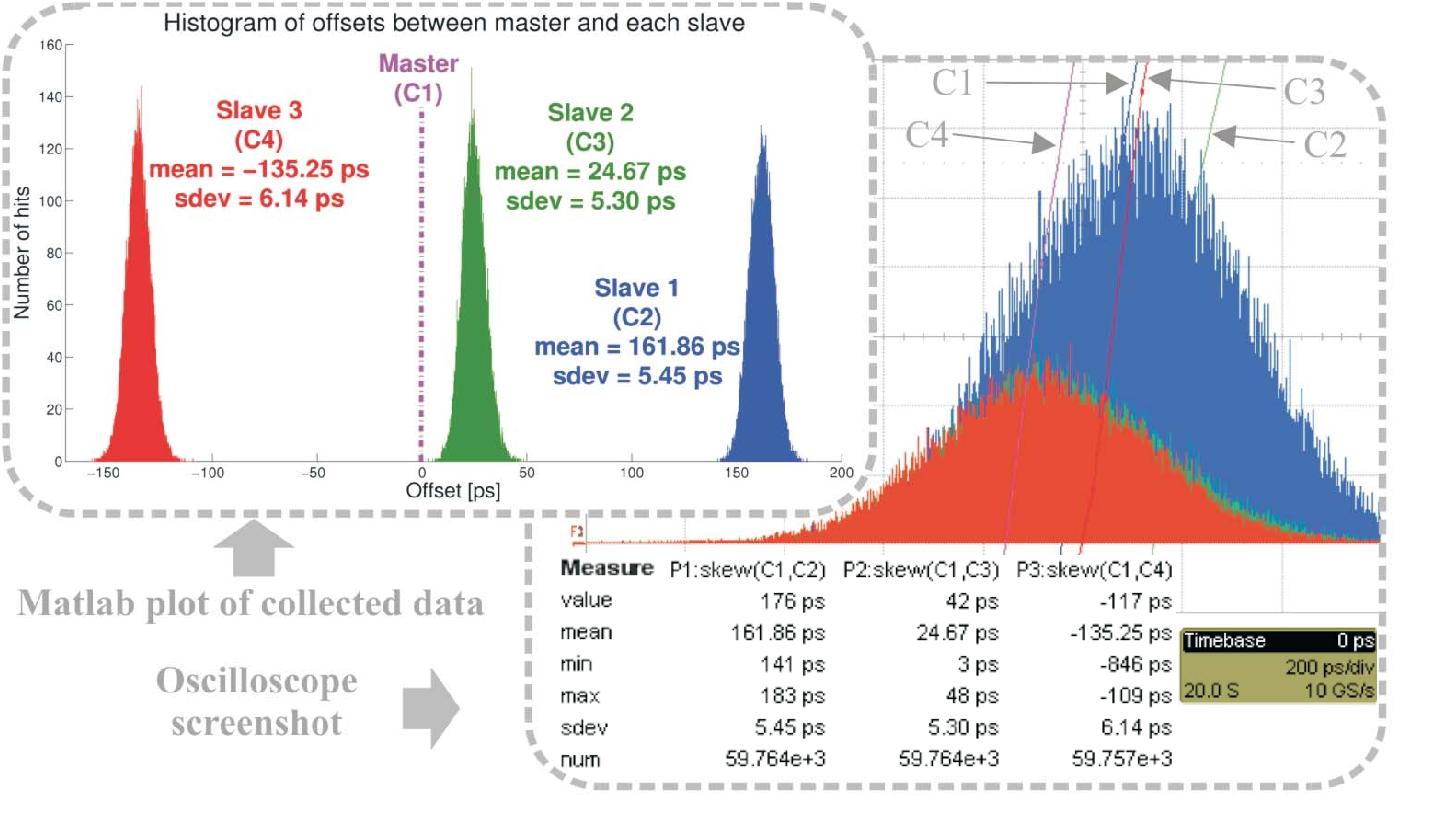
\includegraphics[width=3.4in]{measurements/measResults-new.pdf}
\caption{\modified{Synchronization performance.}}
\label{fig:offset}
\end{figure}

\begin{table}[!t]
\caption{Synchronization and syntonization performance.}
\centering
\begin{tabular}{| c | c |c | c |}          \hline
\multirow{2}{*}{\textbf{Switch}}& 
\textbf{Integrated jitter [ps]}& 
\multicolumn{2}{|c|}{\textbf{Offset [ps]}}  \\ \cline{2-4}
%&   \\ \hline
            & 10Hz-40MHz& mean &  sdev    \\ \hline
            %&   [ps]    &   [ps]     & [ps] & [ps]  & [ps] & [ps]  \\ \hline
1           & 1.6637    &  161.86       &  5.45            \\ \hline
2           & 2.4887    &  24.67        &  5.30            \\ \hline
3           & 2.3025    & -135.25       &  6.14            \\ \hline

\end{tabular}
\label{tab:freqTransfer}
\end{table}
